% Crucial Preamble
\documentclass[12pt,letterpaper]{article} \usepackage{amsmath} \usepackage{graphicx} \usepackage[margin=1in]{geometry} \usepackage{longtable}  \usepackage{amssymb}

% Extra Preamble
\usepackage{fancyhdr} \usepackage{enumitem} \usepackage{float} \usepackage{soul}
\usepackage{multicol} \usepackage[compact]{titlesec} \usepackage{listings}


% frames with display breaks
\usepackage{mdframed}
\allowdisplaybreaks

% change spacing
\usepackage{setspace}
\setlength{\parskip}{0.4\baselineskip}

% Remove paragraph indentation
\setlength{\parindent}{0pt}

% Reduce space before and after section headings
%\titlespacing*{\section}{0pt}{0.1\baselineskip}{0.2\baselineskip}

% changes font
%\renewcommand{\familydefault}{\sfdefault}

% adds header and footer
\pagestyle{fancy}
\fancyhead{} \fancyhead[C]{ADM 1100 Cheat Sheet} \fancyhead[L]{ADM1100} \fancyhead[R]{Owen Daigle}
\fancyfoot{} \fancyfoot[C]{\thepage}


\begin{document}
	
	\begin{center}
		\Large\textbf{ADM 1100 Cheat Sheet} \\
		\vspace{0.5em}
	\end{center}
	
		We are going in a non chronilogical order with the chapters for this course, so the cheat sheet will be in a non chronilogical order as well.
		
		This course is a lot about memorization :-(. 
		
		\section{Chapter 4: Starting a Business}
		
		\subsection{Important Definitions}
		A \textbf{Small Business} is an \textit{owner managed business} with fewer than 100 employees. 
		
		A \textbf{New Venture} is a business opened in the \textit{last 12 months}.
		
		\textbf{Entrepreneurship} is the process of identifying and capitalizing on a marketplace opportunity. 
		
		An \textbf{Entrepreneur} is someone who recognises and seizes oppurtunites. 
		
		An \textbf{Intrapreneur} is someone who creates something new within an existing larg  organization. 
		
		\subsection{Business Plan}
		
		A \textbf{business plan} has the following parts:
		\begin{enumerate}[]\item Cover Page \item Executive Summary (Short overview of the plan)\item Table of Contents\item Company Description (Type, form, of company primary product of company, etc.)\item Product or Serivce Decription (and what is unique about it)\item Marketing (Market Analysis and Plan)\item Operating Plan (Where to get Labour, Raw materials, facilities, etc.)\item Management (Who are they)\item Financial Plan \item Appendix (Extras)\end{enumerate}
		
		\subsection{Alternative Ways of Getting a Business}
		
		\subsubsection{Buying an Existing Business}
		This has \textbf{pros} such as established clients, finances, employees, line of supply, and it is less risky. 
		
		It has \textbf{con} such as being stuck with legacy decision making, financial health, and reputation.
		
		So basically it depends on what the previous owners did to the reputation, could be a good reputation or bad one. 
		
		\subsubsection{Taking over a Family Members Business}
		This can have problems such as who takes over the business, how much it should cost, should other family members automatically get a job, etc. 
		
		\subsubsection{Buying a Franchise}
		This has \textbf{pros} such as expert advice, training provided, low failure rates, and all reputation and stuff is already existing. 
		
		\subsection{Forms of Businesses}
		\begin{center}
			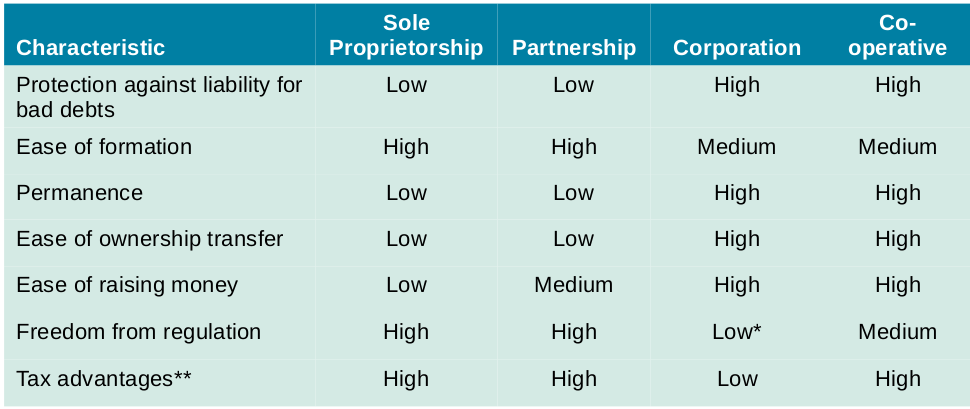
\includegraphics[width=0.7\linewidth]{screenshot001}
		\end{center}
		
		\subsubsection{Sole Proprietorship}
		This basically means that you are in charge of everything. You get to pay minimum fees, do stuff how you want, but if it goes wrong, it is all on you. 
		
		\subsubsection{Partnerships}
		This is when multiple people pool together to share resources, and sometimes liability.
		
		If someone is a \textbf{general partner}, then they share the liability with the other general partners. 
		
		If someone is a \textbf{limited partner}, then they are \textbf{not involved in day to day activities} and do not have any liability.
		
		\subsubsection{Corporation}
		These are \textbf{seperate entities} from the owner. 
		
		If it is \textbf{public}, then anyone can buy shares of the company.
		
		If it is \textbf{private}, then only some people can buy the shares of the company. 
		
		These have limited liabilities for the employees, and professional management, but they have start up costs, and lots of taxation and regulations. 
		
		\subsubsection{Cooperatives}
		These are organiazations created between \textbf{multiple owners} to share supplies. 
		
		They have \textbf{limited liability} for the members, equal voting for all of the members, and there are not many tax problems. 
		
		\section{Chapter 15: Managing Financing}
		\subsection{Short Term Funds}
		Businesses need short term (\textbf{operating}) funds for raw materials, wages, power, rent. 
		
		These can be obtained through trade credit (granting credit to another firm), secured loans (loan with collateral), unsecured loans (loan without collateral) or factoring accounts receivable. 
		
		\subsection{Long Term Funds}
		They also need long term (\textbf{capital}) funds for land, machinery, etc. 
		
		These can be obtained from debt financing (long term loans, or bonds), equity financing (stocks), or hybrid financing (preffered shares are stocks that have no voting rights). 
		
		\subsection{Financial Manager}
		This is a person whose rule is overseeing cash flow management, financial planning, nad financial control.
		
		They obtain funds, manage risk, and conduct the day to day financial activities. 
		
		\subsubsection{Cash Flow Management}
		This is managing the times when the cash is flowing in at a fast rate, and when it is flowing out (not much business).
		
		\subsubsection{Financial Control}
		This is checking the \textbf{performance against plans. }
		
		This is also creating \textbf{budgets} so we don't run out of cash. 
		
		\subsubsection{Financial Planning}
		This is a plan to achieve a desired financial status. 
		
		\subsection{Risk Management}
		Lower risk conserves the firms financial power by minimizing the financial effect of negative events. 
		
		
		\section{Chapter 11: Accounting}
		\textbf{Financial Accounting} keeps external parties informed about the finances. 
		
		\textbf{Managerial Accounting} keeps managers informed about the finances so they can plan.
			
		\subsection{Accounting Equation}
		This equation is: 
		\begin{align*}
			\text{Assets} = \text{Liabilities} + \text{Owners' Equity}
		\end{align*}
		where the assets are anything of economic value, liabilities are any debts, and the owner's equity is any positive difference between the firms assets and liabilities. 
		
		\subsection{Financial Statements}
		
		\subsubsection{Balance Sheets}
		This shows detailed information about \textbf{assets, liabilities, and the owners equity. }
		
		It is a \textbf{snapshot} at a point in time. 
		
		For the assets part of this, we have:
		
		\textbf{Current Assets }are stuff like Cash, Accounts receivable (bills needed to be paid by customers), inventory (unsold merchandise), and prepaid expenses (office supplies, and paid bills such as rent).
		
		\textbf{Fixed assets }have a \textbf{long term value }such as land, buildings, machinery, etc. 
		
		\textbf{Intangible assets }are not physical, but they have a value such as patents, and trademarks. 
		
		\textbf{Goodwill} is also an asset. 
		
		For the liabilities, we have:
		
		\textbf{Current Liabilities} are debts that must be repaid \textbf{within one year.}
		
		\textbf{Long Term liabilities} are debts needed to be repaid in more than one year. 
		
		There is also the \textbf{Owner's Equity} which is the owners holdings in the firm. 
 		\subsubsection{Income Statements}
 		This is the profit and loss statement over a period. 
 		
 		All revnues and expenses are listed including depreciation (value of a building decreases with normal wear and tear).
		
		\subsubsection{Statements of Cash Flow}
		This shows the ccash in, and the cash out from operations, investments, and financing activities. 
		
		\subsection{Financial Ratios}
		There are 3 types of ratios:
		
		Solvency Ratios are the ability to meet total debt obgligations. 
		
		Activity Ratios measure the efficiency in different ways. 
		
		Profitability Ratios measure how well the sales can sustain the business. 
		
		\section{Chapter 10: Operations}
		
		\subsection{Service vs Manufacturing}
		Manufacturing creates a tangable object. 
		
		Service is often not storable and is labour intensive. 
		
		High contact mean that customers MUST be present, while low contact means customers do not need to be physically present. 
		
		The capacity is the amount a firm can produce under normal conditions. 
		
		\subsection{Layouts}
		The process layout groups workers by function or task. This is good for customization.
		
		The product layout gets workers to work in sequential order. This is good for efficiency.
		
		Fixed Position layout balances efficiency and quality. The workers are grouped around the work. 
		
		\subsection{Operations Scheduling}
		The Master OPS Schedule shows which products/services are to be produced over a period and the resources needed. There are detailed (daily, staffing, etc) for specific details. 
		
		We can use GANTT or PERT chart for project scheduling.
		
		\subsection{Productivity}
		This is the ratio between inputs and outputs. 
		
		Just In Time (JIT) production delivers inputs exactly when needed. We do not need to store the inventory.  
		
		\subsection{Total Quality Management TQM}
		This is a model where the quality is the responsability of each worker. Each worker owns the quality of their project. 
		
		\section{Chapter 12/13: Marketing}
		\subsection{Utility} 
		A product/service can offer 4 types of utility:
		\begin{enumerate}[noitemsep]
			\item Time Convenience
			\item Place Convenience
			\item Possession (Such as purchace finance, or product assembly)
			\item Form (Product/service design)
		\end{enumerate}
	
		\subsection{PestG}
		These are the factors that influence a business:
		\begin{enumerate}[noitemsep]
			\item Political Legal (Regulations)
			\item Economic (Effect of the economy)
			\item Social Cultural (Trends going on)
			\item Technological (such as ebooks killing bookstores)
			\item Global (Tariffs and trade agreements)
		\end{enumerate}
	
		\subsection{4 Ps}
		These are the 4 main points of marketing. 
		
		For the \textbf{Price}, the price must be correct .
		
		The \textbf{place} must also be correct, if it is a wrong place, it might be inconvenient for the customer. Also, do we sell direct to customer, through a broker, or to a retail store for them to sell?
		
		Customers might be incentivised to make purchaces if there are \textbf{promotions}.
		
		The actual \textbf{product} must be good. 
		
		\subsection{Market Research}
		To do market research, we can use observation (if we have no idea what is going on), focus group (have a controlled session with customers to discuss and find out stuff), experimentation (we think something will work so we test it in controlled environment) or survey (if we have a pretty good idea of what we need).
		
		\subsection{Product Life Cycle}
		\begin{center}
			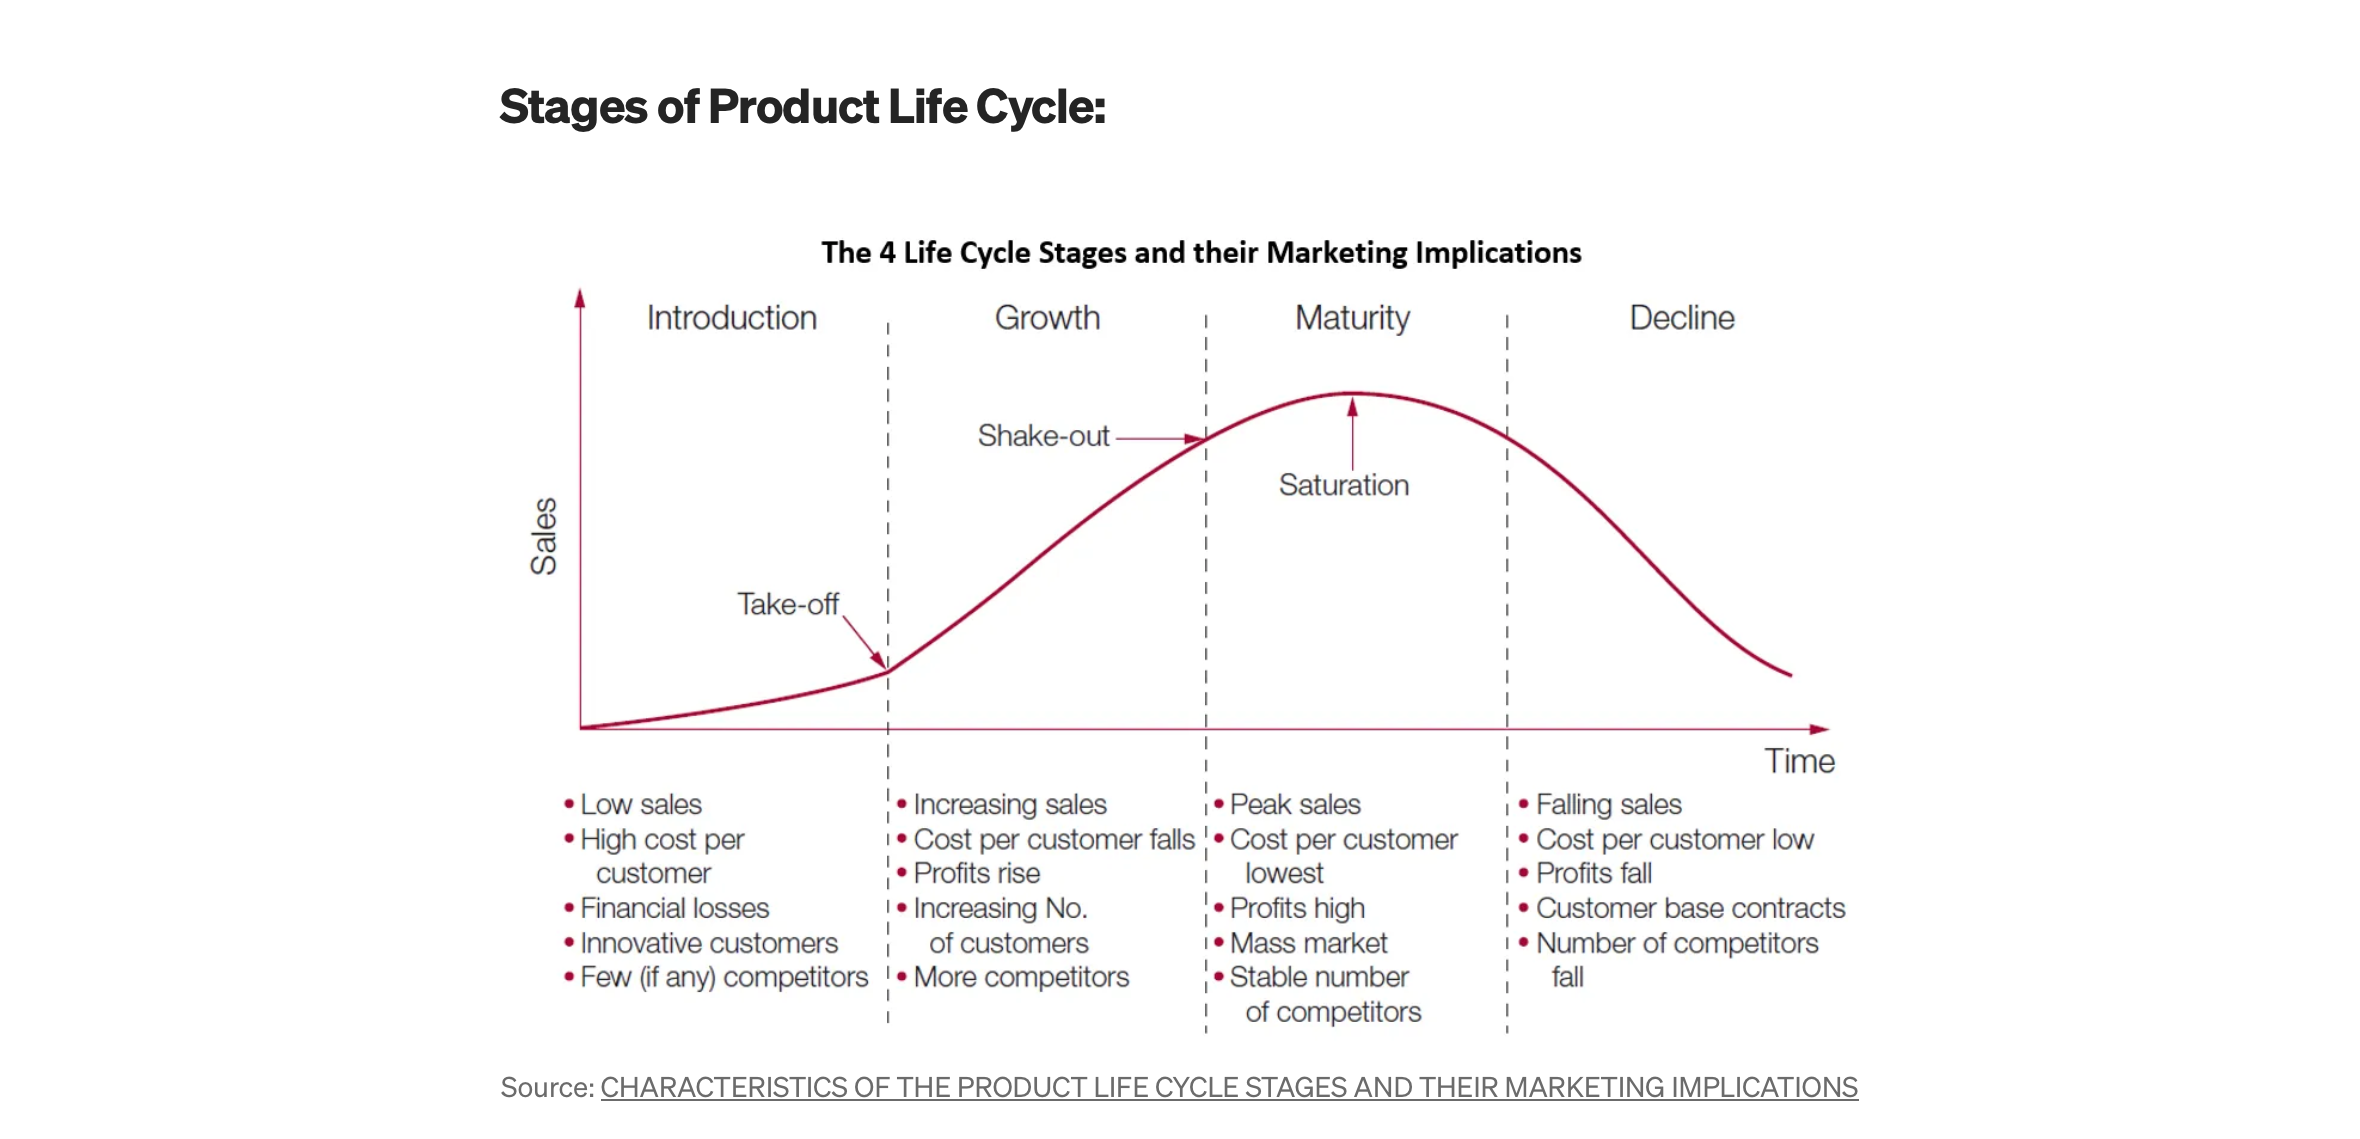
\includegraphics[width=0.9\linewidth]{screenshot002}
		\end{center}

		\subsection{Pricing Strategies}
		We can start by pricing high, and then reducing as more competition emerges. We can also start low (if already lots of competition) and then increase as market share increases.
		
		We can have a fixed price, or change the price as demand goes up.
		
		Price lining is having multiple pricepoints such as "good" "better" "best".
		
		Often we use odd-even pricing (9.99 not 10.00) because of psycology.
		
		Profit Maximising is trying to maximise profit even if we do not sell that many items while Market Share is trying to maximise units sold even if the lower price point means less profit. 
		
		\subsection{Promotion}
		When promoting products, we can use the push strategy by promoting the product to retailers who will then want to stock the product. We can also use the pull strategy which will promote directly to the consumers, and then they will demand the product from the retailers who will buy it. 
		
		The Media Mix is the mix of forms that we use for adertising such as TV, Radio, Newspapers and Internet. 
		
		Promotions are activities designed to stimulate buying such as coupons or purchace incentives. 
		
		Publicity is information made available to consumers by media outlets.
		
		Public relation is company information aimed at building goodwill or dealing with bad events. 
		
		Personal selling is a seller personally interacting with the buyer (such as car dealership)
		
		\subsection{Place}
		A Wholesaler is someone who sells to other businesses. 
		
		A Retailer is someone who sells directly to consumers. 
		
		A Broker issomeone who is hired by the producer to get the products sold. They will communicate with a retailer to sell the item. They match sellers with buyers.
		
		\section{Chapter 6: Managing}
		A Manager is someone who gets stuff done through other people, they rarely do anything directly. 
		
		Top managers have a very conceptual approach, they deal with the overall performance of the firm.
		
		Middle managers implement strategies and work towards the goals set by top managers.
		
		Operations Managers (First line managers) supervise the work of employees that report to them.
		
		Management has the following 4 activities:
		\begin{enumerate}[noitemsep]
			\item Planning (Choose the appropriate organizational goals and courses of action)
			\item Controlling (Evaluate how well we are meeting the goals)
			\item Leading (Motivate, coordinate, and energise individuals)
			\item Organizing (Allocate resources allowing people to work together to achieve the goals)
		\end{enumerate}
	
		SWOT (Strengths Weaknesses, Opportunities Threats) analysis is used to analyse a strategy.
		
		Concentration means growth on a certain one topic. 
		
		Diversification is increasing range of businesses such as expanding to new companies. 
		
		For planning, we have 3 levels:
		\begin{enumerate}[noitemsep]
			\item Strategic Plans (Very long term [3-5 years], Very complex, can have large impact)
			\item Tactical Plans (Medium long term [1-2 years], decently complex, can affect individual businesses but not whole organization drastically)
			\item Operational Plans (Short term, usually focused on one department, the impact is usually very small)
		\end{enumerate}
	
		Contingency Planning is identifying potential threats in the future and ways that the company can respond to those threats.
		
		Crisis management is responding immidiately to an emergency.
	
\end{document}